\section{转录组学概述}
\subsection{概述}
\subsection{定义}
\begin{frame}
  \frametitle{转录组学 | 概述 | 定义 | 基因表达}
  \begin{block}{基因表达}
 基因表达(Gene expression)是用基因中的信息来合成基因产物的过程。产物通常是蛋白质,但对于非蛋白质编码基因,如转运RNA(tRNA)和小核RNA(snRNA),产物则是RNA。\\
 \vspace{0.5em}
基因表达的过程可分为转录、RNA剪接、翻译、蛋白质的翻译后修饰这几步。基因表达调控控制细胞的结构与功能,同时也是细胞分化、形态发生及生物体适应性的基础。不同的时间、不同的环境,以及不同部位的细胞,或是基因在细胞中的含量差异,皆可能使基因产生不同的表现。
  \end{block}
  \begin{figure}
    \centering
    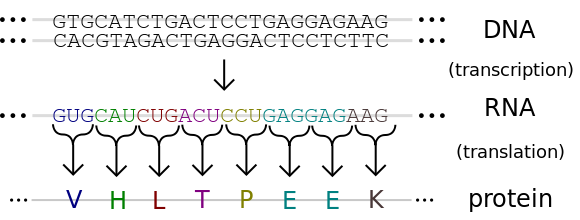
\includegraphics[width=0.7\textwidth]{c3.transcriptome/general.ge.01.png}
  \end{figure}
\end{frame}

\begin{frame}
  \frametitle{转录组学 | 概述 | 定义 | 基因表达谱}
  \begin{block}{基因表达谱}
基因表达谱是一种在分子生物学领域,借助cDNA、表达序列标签(EST)或寡核苷酸芯片来测定细胞基因表达情况(包括特定基因是否表达、表达丰度、不同组织、不同发育阶段以及不同生理状态下的表达差异)的方法。\\
\vspace{1em}
通过一次性测定大量基因构建起细胞功能的总体态势图,可以从图谱中区分出正在分裂的细胞,以及细胞对于特征性治疗的反应。基因表达谱还有助于了解疾病的发病机制、药物的生理反应和治疗效果。\\
\vspace{1em}
基因表达图谱从逻辑上说是基因测序的下一个步骤:基因序列包含细胞可能存在的功能的信息,而基因表达谱则包含细胞实际上正在完成的工作的信息。
  \end{block}
\end{frame}

\begin{frame}
  \frametitle{转录组学 | 概述 | 定义 | 基因表达谱}
  \begin{block}{Technique}
    DNA microarray technology measures the relative activity of previously identified target genes.\\
    \vspace{1em}
 Sequence based techniques, like serial analysis of gene expression (SAGE, SuperSAGE) are also used for gene expression profiling. SuperSAGE is especially accurate and can measure any active gene, not just a predefined set.\\
 \vspace{1em}
 The advent of next-generation sequencing has made sequence based expression analysis an increasingly popular, "digital" alternative to microarrays called RNA-Seq. 
  \end{block}
\end{frame}

\begin{frame}
  \frametitle{转录组学 | 概述 | 定义 | SAGE}
  \begin{block}{SAGE}
    Serial analysis of gene expression (SAGE) is a technique used by molecular biologists to produce a snapshot of the messenger RNA population in a sample of interest in the form of small tags that correspond to fragments of those transcripts.
  \end{block}
  \begin{figure}
    \centering
    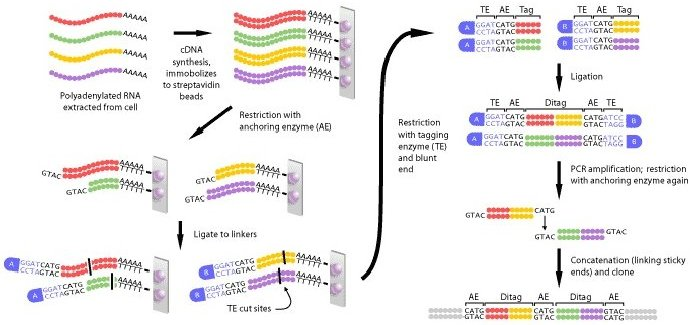
\includegraphics[width=0.8\textwidth]{c3.transcriptome/sage.01.jpg}
  \end{figure}
\end{frame}

\begin{frame}
  \frametitle{转录组学 | 概述 | 定义 | 转录组}
  \begin{block}{转录组}
转录组(Transcriptome),也称为“转录物组”,广义上指在相同环境(或生理条件)下的在一个细胞、或一群细胞中所能转录出的所有RNA的总和,包括信使RNA(mRNA)、核糖体RNA(rRNA)、转运RNA(tRNA)及非编码RNA;狭义上则指细胞所能转录出的所有信使RNA(mRNA)。\\
\vspace{1em}
转录组这个术语可用于指代给定有机体中的转录本总集,或者是特定细胞类型中的特定转录本子集。不考虑突变,固定给定细胞株的基因组数量基本上是不变的;与之不同,转录物组可以随外部环境条件而有所变化。由于转录物组包括了所有在细胞里的mRNA的转录,除却异常的mRNA降解现象(例如转录衰减)以外,转录组反映了在任何给定时间内活跃表达的基因。转录物组学的研究,也被称为“基因表达谱”,检测了在一个特定的细胞群内的mRNA表达水平,通常采用基于DNA微阵列技术的高通量技术。使用新一代测序技术在核苷酸水平上来研究转录物组,被称为“RNA测序(RNA-Seq)”。
  \end{block}
\end{frame}

\begin{frame}
  \frametitle{转录组学 | 概述 | 定义 | 转录组}
  \begin{block}{Methods of construction}
    There are two general methods of inferring transcriptomes.
    \begin{itemize}
      \item One approach maps sequence reads onto a reference genome, either of the organism itself (whose transcriptome is being studied) or of a closely related species.
      \item The other approach, de novo transcriptome assembly, uses software to infer transcripts directly from short sequence reads.
    \end{itemize}
  \end{block}
\end{frame}

\begin{frame}
  \frametitle{转录组学 | 概述 | 定义 | 转录组学}
  \begin{block}{转录组学}
    转录组学(或“转录物组学”)是分子生物学的分支,负责研究在单个细胞或一个细胞群的特定细胞类型内所生产的mRNA分子。\\
    \vspace{1em}
转录组测定的是表达的基因数目。这个数目包括了在各种不同水平上表达的基因。\\
\end{block}
\begin{block}{丰度}
每个细胞里每一种mRNA分子的平均数称为该种mRNA的丰度。根据丰度可把mRNA群体分为两大类:
\begin{itemize}
  \item 高丰度mRNA组分。通常由每个细胞里不到100种的mRNA而每种mRNA分子由1000-10,000份备份所组成,通常占总mRNA的50\%左右。
  \item 除高丰度mRNA组分外,另一半mRNA由长约10,000nt的种类繁多的序列所组成,每种序列在mRNA中只有少量备份。称为“稀有mRNA”或“复杂mRNA”。
\end{itemize}
  \end{block}
\end{frame}

\begin{frame}
  \frametitle{转录组学 | 概述 | 定义 | 转录组学}
大量表达的基因之间是有很大区别的。例如,卵清蛋白只在输卵管细胞里合成而不在肝脏内合成。它占输卵管内mRNA总量的一半。但是高丰度的mRNA只占表达基因数的很小一部分。根据生物体的基因数目以及不同类型细胞出现转录变化的基因数,人们需要了解不同表型细胞稀有mRNA基因相同的程度。\\
\vspace{1em}
稀有mRNA是普遍共有的。一个细胞中的mRNA序列只有10\%左右是该细胞独有的,大部分序列是许多(甚至是所有)类型的细胞所共有的。这提示哺乳动物中共有的基因数也许达10,000个,包括了各种类型细胞所需的功能。编码这种类型的功能的基因,有时被称为“持家基因”或“组成型基因”。这类功能不同于特定细胞表现型所需的特定功能(例如卵清蛋白或珠蛋白的功能)。编码特殊功能的基因称为“奢侈基因”。
\end{frame}

\begin{frame}[label=current]
  \frametitle{转录组学 | 概述 | 定义}
\end{frame}

\subsection{研究方法}

